\section{Преимущества и недостатки систем IOT}
\subsection{Преимущества}
Преимущества IoT охватывают все сферы жизни и бизнеса. Вот список некоторых из
преимущества, которые может предложить IoT:
\begin{itemize}
    \item Улучшение взаимодействия с клиентами. Текущая аналитика страдает от «слепых зон» и
    существенные недостатки в точности; и, как уже отмечалось, взаимодействие остается пассивным. Интернет вещей полностью
    трансформирует это, чтобы добиться более богатого и эффективного взаимодействия с аудиторией.
    \begin{figure}[h!]
        \centering
        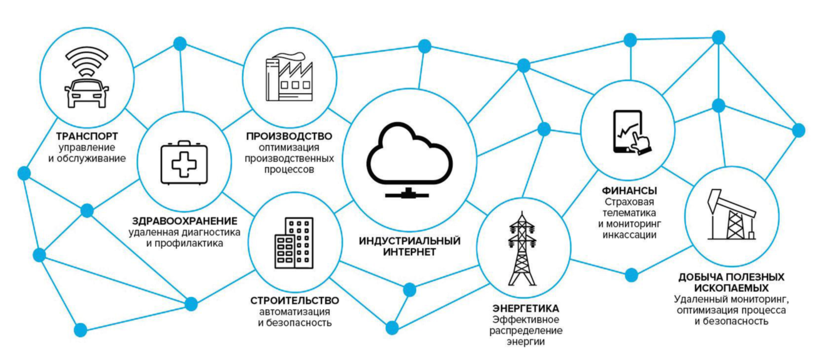
\includegraphics[scale=1]{iot.png}
        \caption{Применение концепции IoT}
        \label{fig:section3:iot}
    \end{figure}
    \item Оптимизация технологий – Те же технологии и данные, которые улучшают
    пользовательских опыт также улучшает использование устройств и помогает в более эффективных улучшениях
    технологии. Интернет вещей открывает мир важных функциональных и полевых данных.
    \item Сокращение отходов – IoT делает очевидными области улучшений. Текущая аналитика дает нам
    поверхностное понимание, но IoT предоставляет реальную информацию, что ведет к более эффективному
    управлению ресурсами.
    \item  Усовершенствованный сбор данных. Современный сбор данных имеет свои ограничения и
    конструкция для пассивного использования. IoT вырывает его из этих пространств и размещает именно там, где
    люди действительно хотят пойти, чтобы проанализировать наш мир. Это позволяет получить точную картину всего.
\end{itemize}
\subsection{Недостатки}
Хотя IoT обеспечивает впечатляющий набор преимуществ, он также сопряжен со значительным набором проблем.
Вот список некоторых его основных проблем:
\begin{itemize}
    \item Безопасность – IoT создает экосистему постоянно подключенных устройств, обменивающихся данными.
    по сетям. Система предлагает мало контроля, несмотря на любые меры безопасности. Это оставляет
    пользователей, подверженных разного рода атакам.
    \item Конфиденциальность — изощренность IoT позволяет предоставлять существенные личные данные в мельчайших подробностях.
    без активного участия пользователя.
    \item Сложность. Некоторые считают системы IoT сложными с точки зрения проектирования, развертывания и
    техническое обслуживание, учитывая их использование нескольких технологий и большого набора новых возможностей
    технологии.
    \begin{figure}[h!]
        \centering
        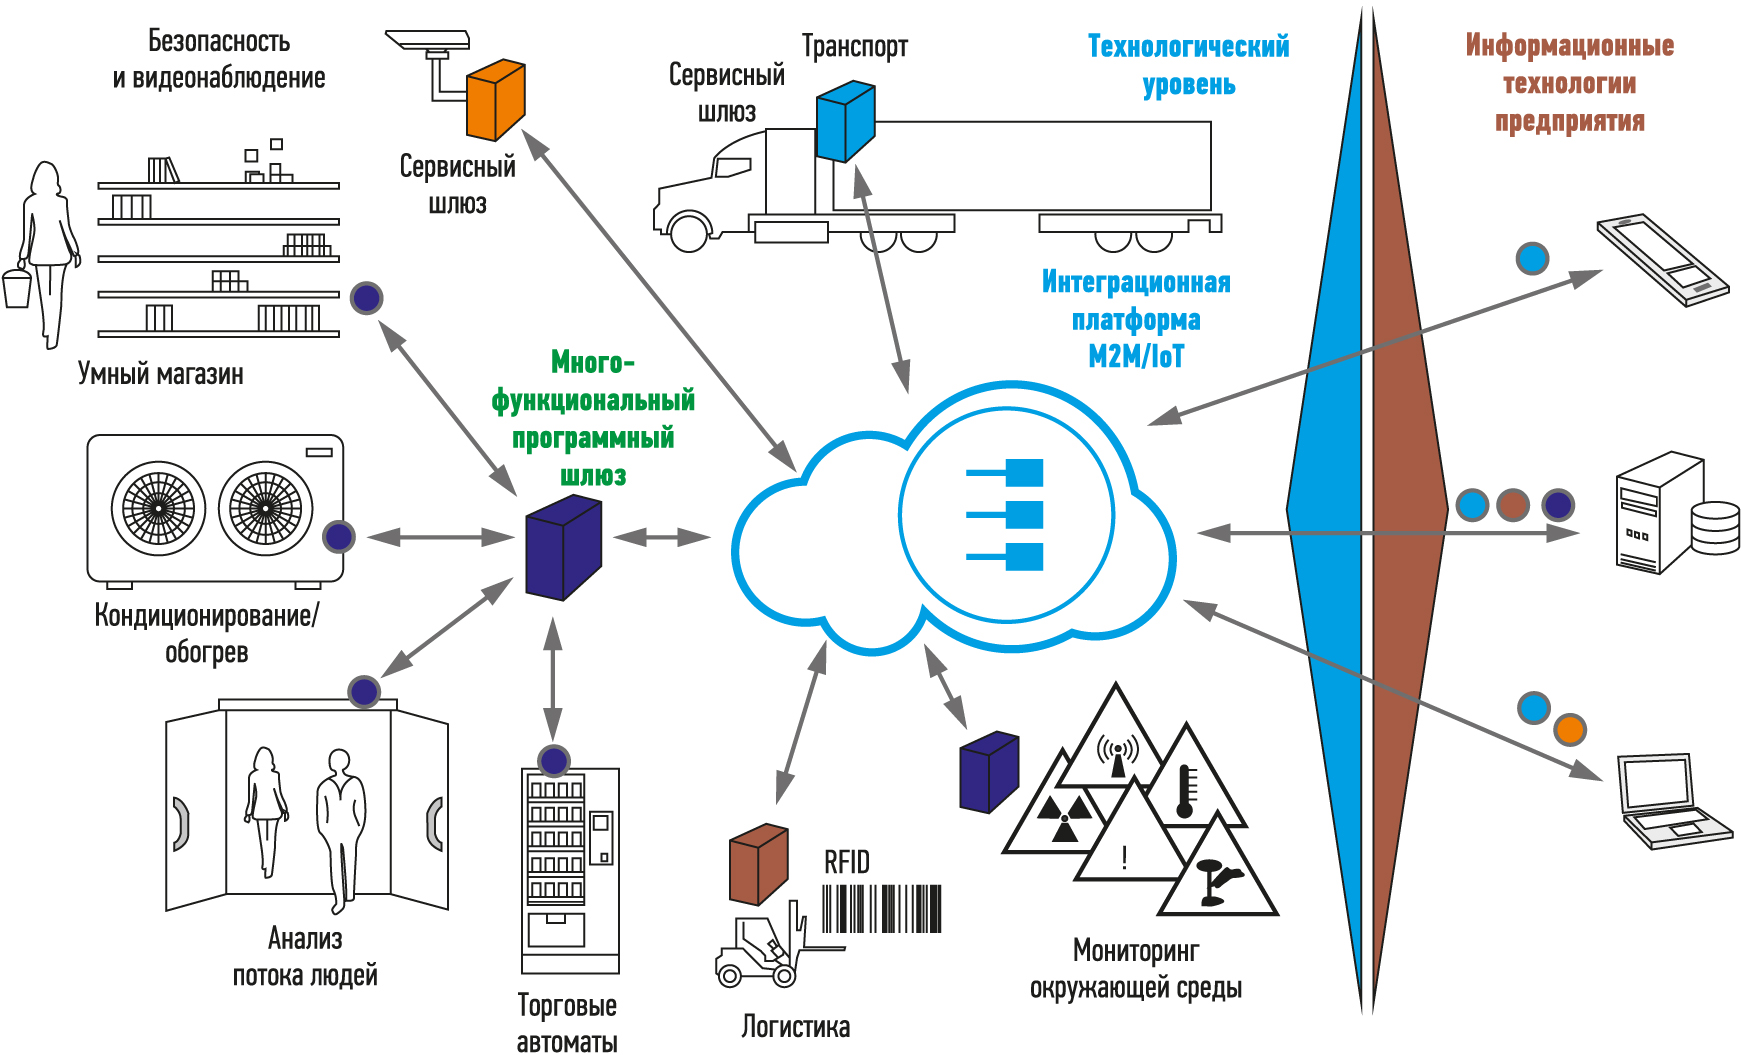
\includegraphics[scale=1]{arch.jpg}
        \caption{Пример архитектуры системы IoT}
        \label{fig:section3:arch}
    \end{figure}
    \item Гибкость. Многих беспокоит гибкость системы IoT для простой интеграции.
    с другим. Они беспокоятся о том, что могут оказаться с несколькими конфликтующими или запертыми
    системы.
    \item Соответствие – IoT, как и любая другая технология в сфере бизнеса, должен соответствовать
    нормативные документы. Его сложность делает вопрос соответствия невероятно сложным
    когда многие считают соответствие стандартного программного обеспечения сражением.
\end{itemize}